\documentclass[tikz,border=2pt]{standalone}
\usepackage{amsmath,amssymb}
\usepackage{tikz}
\usetikzlibrary{arrows.meta,matrix}

\begin{document}
% The identity matrix has 1s on the main diagonal and 0s elsewhere; it leaves every vector
% (and every matrix) unchanged.
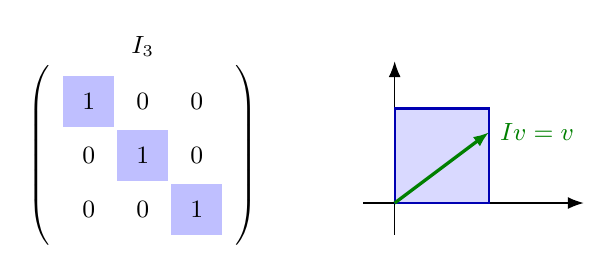
\begin{tikzpicture}[every node/.style={font=\small}, >={Latex[length=2mm]}]
	\matrix (I) [matrix of math nodes, nodes={minimum size=6.5mm, anchor=center}, left delimiter=(, right delimiter=), column sep=1pt, row sep=1pt] at (0,0) {
		|[fill=blue!25]| 1 & 0 & 0 \\
		0 & |[fill=blue!25]| 1 & 0 \\
		0 & 0 & |[fill=blue!25]| 1 \\
	};
	\node[anchor=south] at (I.north) {$I_3$};
	\begin{scope}[xshift=3.2cm, yshift=-0.6cm]
		\draw[->] (-0.4,0) -- (2.4,0);
		\draw[->] (0,-0.4) -- (0,1.8);
		\fill[blue!15] (0,0) rectangle (1.2,1.2);
		\draw[blue!70!black, thick] (0,0) rectangle (1.2,1.2);
		\draw[->, green!50!black, very thick] (0,0) -- (1.2,0.9) node[right] {$Iv=v$};
	\end{scope}
\end{tikzpicture}
\end{document}
